\documentclass[instructions]{StylesAndSettings/uqthesis}
%\documentclass[final]{StylesAndSettings/uqthesis} 

% set how close to the bottom of the page the page number is. Measurement is indicating distance from the last line of text
\setlength{\footskip}{9mm}


%*************************************
% FOR YOUR FINAL THESIS
%*************************************

%IMPORTANT! 
%The default document class (above - line 1 & 2) for the template is \documentclass[instructions]{uqthesis} - this document class will show instructional material and examples relevant to the preliminary material in the compiled PDF preview. THESE INSTRUCTIONS ARE FOR YOUR REFERENCE ONLY AND ARE NOT TO BE INCLUDED IN YOUR FINAL THESIS! 

%To turn off these instructions in your final thesis you MUST use the document class \documentclass[final]{uqthesis} 
%To activate the final thesis document class you must UN-COMMENT THIS DOCUMENT CLASS (remove the % from the start of line 2) and comment out the instructional document class on line 1 (add % to the start of line 1). 

%*************************************
% Introduction to template
%*************************************

%This is The University of Queensland Graduate School Official LaTeX Thesis template.

%Be sure to observe the content of comments within the source code, these are prefaced with a percentage symbol.
%Most important instructions have been CAPITALISED.
%To uncomment an inactive command (if required) remove the % from in front of the command.

%Please see the README for more information.

%This file loads the necessary packages, sets the page styles, and defines required macros.
%Edit this if you are comfortable with LaTeX.

%Other tweaks can be made in StylesAndSettings/uqthesis.cls, but change these at your own risk!

%See README for version.

%You must have the memoir class installed.

% ***************************************************
% LaTeX Packages
% ***************************************************
% This file defines the document design.
% Usually it is not necessary to edit this file, but you can use it to change aspects of the design if you want.

%There are essential packages that are contained within the StylesAndSettings/uqthesis.cls which are integral to the template - These must not be deleted.

%The packages below are optional, please add or alter as required.

\usepackage{cite}				 %Allows abbreviated numerical citations.
\usepackage{pdfpages}			 %Allows you to include full-page pdfs.
\usepackage{wrapfig}			 %Lets you wrap text around figures.
\usepackage{bm} 				 %Bolded maths characters.
\usepackage{upgreek}			 %Upright Greek characters.
\usepackage{dsfont}				 %Double-struck fonts.
\usepackage{simplewick}			 %For typesetting Wick contractions.
\usepackage{mathtools}		     %Can be used to fine-tune the maths presentation.	
\usepackage{framed}			     %For boxed text.
\usepackage{microtype}			 %pdfLaTeX will fix your kerning.
\usepackage{marvosym}			 %Include symbols (like the Euro symbol, etc.).
\usepackage{color}				 %Nice for scalable pdf graphics using Inkscape.
\usepackage{transparent}	     %Nice for scalable pdf graphics using Inkscape.
\usepackage{placeins}			 %Lets you put in a \FloatBarrier to stop figures floating past this command.
\usepackage{mdframed,mdwlist}    %Use these for nice lists (less white space).
\usepackage{float}               %Improved interface for floating objects. 
\usepackage{mathdots}            %Changed the basic LaTeX and plain TeX commands.
\usepackage{eucal}               %Font shape definitions to use the Euler script symbols in math mode.
\usepackage{array}               %Extending the array and tabular environments.
\usepackage{stmaryrd}            %The StMary’s Road symbol font.
\usepackage{pifont}              %Access to PostScript standard Symbol and Dingbats fonts.
\usepackage{lipsum}              %Easy access to the Lorem Ipsum sample text.
\usepackage{enumerate}           %Enumerate with redefinable labels.
\usepackage[all]{xy}             %This is a special package for drawing diagrams.
\usepackage[utf8]{inputenc}      %Makes all displayable utf8 characters available as input.
\usepackage{fancyhdr}            %Extensive control of page headers and footers.
\usepackage{blindtext}           %Produced 'blind' text for testing.
\usepackage{tikz}                %To create graphic elements.
\usetikzlibrary{shapes.geometric, arrows.meta, positioning, calc}
\usepackage[figuresright]{rotating}	%Allows large tables to be rotated to landscape.
\usepackage{chngcntr} % Allows tables to not include chapter numbers
%You can add more packages here if you need
\usepackage{caption} % Allows caption formatting to be customised
\usepackage{titlesec} % Added for changing heading and title spacing


%This defines some macros that implement Latin abbreviations
%COMMENT OUT OR DELETE IF UNDESIRED.
\newcommand{\via}{\textit{via}} %Italicised via.
\newcommand{\ie}{\textit{i.e.}} %Literally.
\newcommand{\eg}{\textit{e.g.}} %For example.
\newcommand{\etc}{\textit{etc.}} %So on...
\newcommand{\vv}{\textit{vice versa}} %And the other way around.
\newcommand{\viz}{\textit{viz}.} %Resulting in.
\newcommand{\cf}{\textit{cf}.} %See, or 'consistent with'.
\newcommand{\apr}{\textit{a priori}} %Before the fact.
\newcommand{\apo}{\textit{a posteriori}} %After the fact.
\newcommand{\vivo}{\textit{in vivo}} %In the flesh.
\newcommand{\situ}{\textit{in situ}} %On location.
\newcommand{\silico}{\textit{in silico}} %Simulation.
\newcommand{\vitro}{\textit{in vitro}} %In glass.
\newcommand{\vs}{\textit{versus}} %James \vs{} Pete.
\newcommand{\ala}{\textit{\`{a} la}} %In the manner of...
\newcommand{\apriori}{\textit{a priori}} %Before hand.
\newcommand{\etal}{\textit{et al.}} %And others, with correct punctuation.
\newcommand{\naive}{na\"\i{}ve} %Queen Amidala is young and \naive{}.


% ***************************************************
% Title page
% ***************************************************

%***THESIS TITLE***
%Use Sentence Case (capitalise only the first word and proper nouns).
\title{Reinforcement Learning for Control of Robotic Perception Systems}

%***YOUR NAME***
%Do not include initials or middle names. Do not include your supervisor(s)' name(s).
\author{Santiago Rodrigues}
%***YOUR CURRENT DEGREES***
%Use abbreviations. Do not include the date or location of your degree. Do not include the degree for which this thesis is being submitted.
% \currentdegrees{Candidate’s academic degrees}

%***ORCID ID***
%Add and hyperlink your ORCID
\orcid{\href{add your ORCID url here}{Candidate's ORCID}}

%***YEAR OF SUBMISSION***
\date{2025}
%***TYPE OF DEGREE***
\submittedfor{Bachelors of Engineering (Honours) and Computer Science}


%***YOUR SCHOOL***
%Use Title Case (capitalise every word which is not a conjunction or preposition).
%See - https://blog.apastyle.org/apastyle/2012/03/title-case-and-sentence-case-capitalization-in-apa-style.html - for help.
\school{METR4911}


%HBAR fix added by Michael
% (this issue is related to the use of the mathptmx package)
\begin{document}
\renewcommand{\hbar}{\mathchar'26\mkern-7.5mu h}


\frontmatter
% Assemble title page
\maketitle
\clearpage
\setcounter{page}{1}

% ***************************************************
% How to Use this Template Page - This Section Will be hidden when you change the document class
%****************************************************

\begin{instructional}
\pagestyle{plain}
% \section*{How to Use this Template}
\normalfont
%Open abstract.tex to edit
%% ***************************************************
% How to Use this Template
% ***************************************************

% \noindent
% \textbf{\large Title Page}
% \begin{itemize}
%     \item Replace text enclosed in curly brackets \{ \} with your own content.
%     \item The thesis title should be formatted in sentence case (i.e. only the first word and proper nouns should be capitalised).
%     \item Present your name as it appears in your official UQ MySI-net record. Official name changes can be made through \href{https://my.uq.edu.au/contact/student-central}{\color{blue}{UQ Student Central}}.
%     \item The degrees listed must be tertiary degrees that have already been awarded. The name of the institution is not required. You cannot list the degree currently being examined.
%     \item Include the year of submission (month/day is not required).
%     \item List your enrolling unit. If you have any non-enrolling units (e.g., Centres), they must be placed on a new line below the enrolling unit’s name.
%     \item The UQ logo provided on the Title Page has been approved by UQ for use in all HDR theses. Other versions of the UQ logo will not be accepted. Please do not change the size of the logo.
%     \item You may add one additional image on the title page, provided it is small enough not to overwhelm the title information. Obtain copyright permission before inserting any image, and note any AI-generated images in the preliminary pages.
%     \item Please do not add any other content or change the formatting of the Title Page.
% \end{itemize}

% \vspace{0.3em}

% \noindent
% \textbf{\large Preliminary Pages}   
% \begin{itemize}
% \itemsep0em 
%     \item Do not modify the wording or format of any headings on the preliminary pages.
%     \item Retain all headings in the order provided in this template.
%     \item Replace text enclosed in curly brackets \{ \} with your own content.
%     \item Delete or replace any instructional text (displayed in purple) before submitting your thesis. In LaTeX you can quickly achieve this following the Instructions in MainThesis.tex.
%     % This instruction was given extra clarification for LaTeX use.
% \end{itemize}

% \vspace{0.3em}

% \noindent
% \textbf{\large Thesis Content Pages}   
% \begin{itemize}
% \itemsep0em 
%     \item The remainder of the template starting with ‘Table of Contents’ is offered as guidance only and is not intended to be prescriptive. You may adapt it to suit your discipline's requirements and conventions.
%     %Talking about Microsoft styles doesn't make sense for a LaTeX template, however it's not as easy as deleting this item because it also talks about auto-numbering
%     %\item The content pages that follow the preliminary pages are formatted using Microsoft Styles with embedded auto-numbering for chapters and headings. Page numbers have been incorporated to enable the automatic generation of the Table of Contents, as well as lists of tables and figures.
%     \item The content pages that follow the preliminary pages are formatted using styles defined in the uqthesis.cls class file, including auto-numbering for chapters and headings. Page numbers have been incorporated for the Table of Contents, as well as lists of tables and figures.
%     \item Following publishing conventions, this template uses Roman numerals for the preliminary pages and Arabic numerals for the main body. Adjust the numbering as required by your discipline; however, please ensure that the title page does not display a page number.
%     \item Mark each blank page in your thesis with: ``This page was intentionally left blank."
% \end{itemize}

% \clearpage
% \noindent
% \textbf{\large \LaTeX \,Instructions}

% \noindent
% This template has been designed with Overleaf, but can be used with a local distribution.
% \begin{itemize}
%     \item Compile \textbf{MainThesis.tex}, ensuring that you have all of the necessary packages.
%     \item Add or subtract packages in LaTexPackages.tex as needed for your thesis.
%     %Can this be reworded, or removed?
%     \item Insert the appropriate bibstyle and .bib files into MainThesis.tex to allow BibTeX to function correctly. A References.bib file, which you may use or replace, is in the \textbf{/References/} directory.
%     \item Add each chapter as a separate .tex file using input commands in MainThesis.tex. 
%     \item Chapter.tex files and associated figures should be kept in their own directory. 
%     \item Complete your list of abbreviations and symbols in Preliminary.tex. You may add TeX packages to assist this process.
%     \item When ready to submit, ensure that the document class in MainThesis.text is \textbf{final}, not \textbf{instructions}. This can be changed on lines 1 and 2.
% \end{itemize}

% \vspace{0.4em}

% \noindent
% \textbf{\large \LaTeX \,Files}

% \begin{itemize}
%     \item MainThesis.tex is the main file which receives the others as inputs.
%         \item The \textbf{/PreliminaryPages/} directory contains three .tex files: 
%         \begin{itemize}[after=\vspace{0pt}]
%         \item Abstract.tex contains instructions for compiling a stand-alone version of the abstract for submission purposes.
%         \item Authordeclaration.tex is the author declaration that must appear \textbf{verbatim} in your final thesis. \\ DO NOT EDIT!
%         \item Preliminary.tex contains the front matter, everything prior to the body of the document.     
%         \end{itemize}
%     \item The \textbf{/StylesAndSettings/} directory contains files to control various styling and settings
%         \begin{itemize}[after=\vspace{0pt}] 
%         \item uqthesis.cls loads necessary packages, sets page and heading styles, defines the line spread and redefines the $\sqrt{}$ command to improve readability by adjusting white space.
%         \item uqtitle.sty sets the title page style and defines storage commands, etc.
%         \item LaTexPackages.tex defines optional packages and text macros.
%         \item UQLogo.jpg is the UQ shield logo.
%         \item OrcidLogo.jpg is the Orcid logo.
%         \item abbrv-unsrt.bst is a numerical bibliographic citation style by E. Krepska providing short numerical citations in citation order. This is an example, you may choose your preferred or required style.
%         \item GNU\_License.txt is a copy of the GNU General Public License v3.
%         \end{itemize}


%     \item The \textbf{/Examples/} directory is for reference only. DO NOT INCLUDE any of these files in your thesis.
% \end{itemize}


% \noindent
% For further tips and advice, please see \href{https://my.uq.edu.au/information-and-services/higher-degree-research/my-thesis}{\color{blue}{UQ’s HDR Thesis Advice}}. If you have any questions regarding the template format or the required headings, please contact the UQ Graduate School via \href{mailto:graduateschool@uq.edu.au}{\color{blue}{graduateschool@uq.edu.au}}. The Library offers help with formatting via \href{mailto:training@library.uq.edu.au?subject=Overleaf Thesis Template help}{\color{blue}{training@library.uq.edu.au}}.

% ***************************************************

%\end{document}


%*************************************
%*****UQ LaTeX THESIS TEMPLATE********
%*************************************
% Copyright (C) 2025 The University of Queensland Graduate School
% Last revision: 23 May 2025.

%*************************************
%*************LICENSING:**************
%*************************************

%The User acknowledges the existence of and agrees to comply with all relevant terms and conditions. In particular:

%a.	The Graduate Thesis Template has been created using open-source software, the terms of which can be found below;
%b.	Access to the Template through editor programs such as Overleaf requires compliance with the terms and conditions governing those editor programs. 
%c.	The Template contains content that is the intellectual property of The University of Queensland, including copyright and protected marks, which must be respected in accordance with applicable laws;
%d.	The University of Queensland does not collect any private data arising from the use of the Graduate Thesis Template.

%This program is free software: you can redistribute it and/or modify it under the terms of the GNU General Public License (GNU License can be located under the /StylesAndSettings/GNU_License.txt file) as published by the Free Software Foundation, either version 3 of the License, or (at your option) any later version.

%This program is distributed in the hope that it will be useful, but WITHOUT ANY WARRANTY; without even the implied warranty of MERCHANTABILITY or FITNESS FOR A PARTICULAR PURPOSE. See the GNU General Public License for more details. You should have received a copy of the GNU General Public License along with this program. If not, see <https://www.gnu.org/licenses/>.

%*************************************
%**********ACKNOWLEDGEMENTS:**********
%*************************************

%The latest version of this template has been updated by The University of Queensland Library. Thank you to Nicholas Wiggins, Cameron West, Stéphane Guillou, David Miles, Luke Gaiter and Michael Feeney for your involvement with this update.

%Previous contributors include Elena Danilova, Trinity McNicol, James Nicholson, Hanna Reinebrant, Sanjib Mondal, Jan Mairhoefer, Preeti Vayada, Nick Fitt, Paul Cochrane, Will Petterrsen, James Bennett, Christiaan Bekker, Thomas Bell, Catxere Andrade Casacio, Nicolas Mauranyapin, Varun Prakash, and Alexander Stilgoe.

% ***************************************************

%\end{document}
% ***************************************************
% How to Use this Template
% ***************************************************

% \noindent
% \textbf{\large Title Page}
% \begin{itemize}
%     \item Replace text enclosed in curly brackets \{ \} with your own content.
%     \item The thesis title should be formatted in sentence case (i.e. only the first word and proper nouns should be capitalised).
%     \item Present your name as it appears in your official UQ MySI-net record. Official name changes can be made through \href{https://my.uq.edu.au/contact/student-central}{\color{blue}{UQ Student Central}}.
%     \item The degrees listed must be tertiary degrees that have already been awarded. The name of the institution is not required. You cannot list the degree currently being examined.
%     \item Include the year of submission (month/day is not required).
%     \item List your enrolling unit. If you have any non-enrolling units (e.g., Centres), they must be placed on a new line below the enrolling unit’s name.
%     \item The UQ logo provided on the Title Page has been approved by UQ for use in all HDR theses. Other versions of the UQ logo will not be accepted. Please do not change the size of the logo.
%     \item You may add one additional image on the title page, provided it is small enough not to overwhelm the title information. Obtain copyright permission before inserting any image, and note any AI-generated images in the preliminary pages.
%     \item Please do not add any other content or change the formatting of the Title Page.
% \end{itemize}

% \vspace{0.3em}

% \noindent
% \textbf{\large Preliminary Pages}   
% \begin{itemize}
% \itemsep0em 
%     \item Do not modify the wording or format of any headings on the preliminary pages.
%     \item Retain all headings in the order provided in this template.
%     \item Replace text enclosed in curly brackets \{ \} with your own content.
%     \item Delete or replace any instructional text (displayed in purple) before submitting your thesis. In LaTeX you can quickly achieve this following the Instructions in MainThesis.tex.
%     % This instruction was given extra clarification for LaTeX use.
% \end{itemize}

% \vspace{0.3em}

% \noindent
% \textbf{\large Thesis Content Pages}   
% \begin{itemize}
% \itemsep0em 
%     \item The remainder of the template starting with ‘Table of Contents’ is offered as guidance only and is not intended to be prescriptive. You may adapt it to suit your discipline's requirements and conventions.
%     %Talking about Microsoft styles doesn't make sense for a LaTeX template, however it's not as easy as deleting this item because it also talks about auto-numbering
%     %\item The content pages that follow the preliminary pages are formatted using Microsoft Styles with embedded auto-numbering for chapters and headings. Page numbers have been incorporated to enable the automatic generation of the Table of Contents, as well as lists of tables and figures.
%     \item The content pages that follow the preliminary pages are formatted using styles defined in the uqthesis.cls class file, including auto-numbering for chapters and headings. Page numbers have been incorporated for the Table of Contents, as well as lists of tables and figures.
%     \item Following publishing conventions, this template uses Roman numerals for the preliminary pages and Arabic numerals for the main body. Adjust the numbering as required by your discipline; however, please ensure that the title page does not display a page number.
%     \item Mark each blank page in your thesis with: ``This page was intentionally left blank."
% \end{itemize}

% \clearpage
% \noindent
% \textbf{\large \LaTeX \,Instructions}

% \noindent
% This template has been designed with Overleaf, but can be used with a local distribution.
% \begin{itemize}
%     \item Compile \textbf{MainThesis.tex}, ensuring that you have all of the necessary packages.
%     \item Add or subtract packages in LaTexPackages.tex as needed for your thesis.
%     %Can this be reworded, or removed?
%     \item Insert the appropriate bibstyle and .bib files into MainThesis.tex to allow BibTeX to function correctly. A References.bib file, which you may use or replace, is in the \textbf{/References/} directory.
%     \item Add each chapter as a separate .tex file using input commands in MainThesis.tex. 
%     \item Chapter.tex files and associated figures should be kept in their own directory. 
%     \item Complete your list of abbreviations and symbols in Preliminary.tex. You may add TeX packages to assist this process.
%     \item When ready to submit, ensure that the document class in MainThesis.text is \textbf{final}, not \textbf{instructions}. This can be changed on lines 1 and 2.
% \end{itemize}

% \vspace{0.4em}

% \noindent
% \textbf{\large \LaTeX \,Files}

% \begin{itemize}
%     \item MainThesis.tex is the main file which receives the others as inputs.
%         \item The \textbf{/PreliminaryPages/} directory contains three .tex files: 
%         \begin{itemize}[after=\vspace{0pt}]
%         \item Abstract.tex contains instructions for compiling a stand-alone version of the abstract for submission purposes.
%         \item Authordeclaration.tex is the author declaration that must appear \textbf{verbatim} in your final thesis. \\ DO NOT EDIT!
%         \item Preliminary.tex contains the front matter, everything prior to the body of the document.     
%         \end{itemize}
%     \item The \textbf{/StylesAndSettings/} directory contains files to control various styling and settings
%         \begin{itemize}[after=\vspace{0pt}] 
%         \item uqthesis.cls loads necessary packages, sets page and heading styles, defines the line spread and redefines the $\sqrt{}$ command to improve readability by adjusting white space.
%         \item uqtitle.sty sets the title page style and defines storage commands, etc.
%         \item LaTexPackages.tex defines optional packages and text macros.
%         \item UQLogo.jpg is the UQ shield logo.
%         \item OrcidLogo.jpg is the Orcid logo.
%         \item abbrv-unsrt.bst is a numerical bibliographic citation style by E. Krepska providing short numerical citations in citation order. This is an example, you may choose your preferred or required style.
%         \item GNU\_License.txt is a copy of the GNU General Public License v3.
%         \end{itemize}


%     \item The \textbf{/Examples/} directory is for reference only. DO NOT INCLUDE any of these files in your thesis.
% \end{itemize}


% \noindent
% For further tips and advice, please see \href{https://my.uq.edu.au/information-and-services/higher-degree-research/my-thesis}{\color{blue}{UQ’s HDR Thesis Advice}}. If you have any questions regarding the template format or the required headings, please contact the UQ Graduate School via \href{mailto:graduateschool@uq.edu.au}{\color{blue}{graduateschool@uq.edu.au}}. The Library offers help with formatting via \href{mailto:training@library.uq.edu.au?subject=Overleaf Thesis Template help}{\color{blue}{training@library.uq.edu.au}}.

% ***************************************************

%\end{document}


%*************************************
%*****UQ LaTeX THESIS TEMPLATE********
%*************************************
% Copyright (C) 2025 The University of Queensland Graduate School
% Last revision: 23 May 2025.

%*************************************
%*************LICENSING:**************
%*************************************

%The User acknowledges the existence of and agrees to comply with all relevant terms and conditions. In particular:

%a.	The Graduate Thesis Template has been created using open-source software, the terms of which can be found below;
%b.	Access to the Template through editor programs such as Overleaf requires compliance with the terms and conditions governing those editor programs. 
%c.	The Template contains content that is the intellectual property of The University of Queensland, including copyright and protected marks, which must be respected in accordance with applicable laws;
%d.	The University of Queensland does not collect any private data arising from the use of the Graduate Thesis Template.

%This program is free software: you can redistribute it and/or modify it under the terms of the GNU General Public License (GNU License can be located under the /StylesAndSettings/GNU_License.txt file) as published by the Free Software Foundation, either version 3 of the License, or (at your option) any later version.

%This program is distributed in the hope that it will be useful, but WITHOUT ANY WARRANTY; without even the implied warranty of MERCHANTABILITY or FITNESS FOR A PARTICULAR PURPOSE. See the GNU General Public License for more details. You should have received a copy of the GNU General Public License along with this program. If not, see <https://www.gnu.org/licenses/>.

%*************************************
%**********ACKNOWLEDGEMENTS:**********
%*************************************

%The latest version of this template has been updated by The University of Queensland Library. Thank you to Nicholas Wiggins, Cameron West, Stéphane Guillou, David Miles, Luke Gaiter and Michael Feeney for your involvement with this update.

%Previous contributors include Elena Danilova, Trinity McNicol, James Nicholson, Hanna Reinebrant, Sanjib Mondal, Jan Mairhoefer, Preeti Vayada, Nick Fitt, Paul Cochrane, Will Petterrsen, James Bennett, Christiaan Bekker, Thomas Bell, Catxere Andrade Casacio, Nicolas Mauranyapin, Varun Prakash, and Alexander Stilgoe.

% ***************************************************

%\end{document}

\clearpage
\end{instructional}
% ***************************************************

% ***************************************************
% Preface
%****************************************************
\pagestyle{plain}
\section*{Abstract}
\normalfont
%Open abstract.tex to edit
\input{./PreliminaryPages/Abstract.tex}

\clearpage
% ***************************************************
\section*{Declaration by Author}
%DO NOT EDIT.
\input{./PreliminaryPages/Authordeclaration.tex}

\clearpage
%YOU MUST EDIT THIS DOCUMENT.
% Requires: \usepackage{colortbl}
% ***************************************************
% PRELIMINARY PAGES
% ***************************************************
% The instructions contained within this part of the thesis template need to be suppressed from the final thesis. There are instructions on how to do this in the MainThesis.tex file.

% To ensure your work is not suppressed with the instructions please add your text only where instructed.


%***Publications Included in this Thesis***
% \section*{Publications Included in this Thesis}
% \begin{instructional}
% 	Start this section on a new page [this template will automatically handle this].\\
    
% 	\noindent
%     If you choose to include publications as part of your thesis as described in the UQ \href{https://policies.uq.edu.au/document/view-current.php?id=452}{\color{blue}{HDR Examination Guidelines}} use this section to list any publications included in this thesis using the appropriate \href{https://guides.library.uq.edu.au/referencing}{\color{blue}{referencing style}} for your discipline. If in doubt, seek advice from your advisory team.\\

% 	\noindent
%     Arrange your publications under the following four sub-headings:
%     \begin{itemize}
%         \item \textbf{Published}: Any publications that have been formally published.
%         \item \textbf{Accepted}: Publications that have been accepted or are in press.
%         \item \textbf{Submitted}: Manuscripts submitted for publication that are currently awaiting review outcomes.
%         \item \textbf{Drafted}: Manuscripts that are in draft form.\\
%     \end{itemize}

%     \noindent
% 	Exclude any sub-headings that are not relevant. If you have not included any of your publications in the thesis then state ``No publications included''.\\

    
%     \noindent
%     Additional important considerations:
% 	\begin{enumerate}
% 		\item	Research contributing to scholarly work that is included in the thesis must have been conducted during candidature. Works published prior to or after candidature cannot be included in the thesis.
% 		\item	At a minimum, any thesis that includes publications must contain:
%             \begin{itemize}[after=\vspace{0pt}] 
%                 \item an independent introduction that contextualises the research project in relation to the present state of the knowledge in the field
%                 \item thesis chapters (i.e. publications) in a logical and cogent sequence leading to an argument that supports the main findings of the thesis
%                 \item an independent and original discussion that integrates the significant findings of the thesis.
%             \end{itemize}
% 		\item	Accepted or published works included in the thesis must be presented as the final author-submitted manuscript, not in the journal's published format.		\item	Permission must be obtained to reproduce copyright material in the thesis unless, as part of the publication process, permission has already been granted. A statement attesting to copyright permission must be explicitly included in the thesis.	
%         \item	The presence of peer-reviewed published works within the thesis does not pre-empt or negate the examiners' assessment of the quality of this work within the thesis, nor does it preclude amendments to the thesis based on the examiners' feedback.
% 	\end{enumerate}
	
% \end{instructional}

% ********* Enter your text below this line: ********


% ***************************************************


%***Other Publications During Candidature***
% \section*{Other Publications During Candidature}

% \begin{instructional}
%     List other publications authored during your candidature that are not included in this thesis using the appropriate \href{https://guides.library.uq.edu.au/referencing}{\color{blue}{referencing style}} for your discipline. If in doubt, seek advice from your advisory team.\\


%     \noindent
%     Arrange your publications under the following four sub-headings:
%     \begin{itemize}
%         \item \textbf{Published}: Any publications that have been formally published.
%         \item \textbf{Accepted}: Publications that have been accepted or are in press.
%         \item \textbf{Submitted}: Manuscripts submitted for publication that are currently awaiting review outcomes.
%         \item \textbf{Drafted}: Manuscripts that are in draft form.
%     \end{itemize}
    
%     \noindent
% 	Exclude any sub-headings that are not relevant. If you have not included any of your publications in the thesis then state ``No publications included''.\\


% \end{instructional}

% ********* Enter your text below this line: ********


% ***************************************************


\clearpage
%***Contributions by Others to this Thesis***
% \section*{Contributions by Others to this Thesis}

% \begin{instructional}

% 	Start this section on a new page [this template will automatically handle this].\\

% 	\noindent
% 	The HDR thesis must be your original work. You must explicitly acknowledge any contributions or support received from others, clearly indicating the nature and extent of their involvement. Your contributions to each chapter must satisfy the University’s \href{https://policies.uq.edu.au/document/view-current.php?id=377}{\color{blue}{Authorship Procedure}} and the \href{https://policies.uq.edu.au/document/view-current.php?id=248}{\color{blue}{HDR Examination Procedure}}.  \\

%     \noindent
%     Your contribution should be substantial and cover at least one, and usually several, of the following areas:
%     \begin{enumerate}
%         \item conception and design of the project;
%         \item acquisition of research data where the acquisition has required significant intellectual judgement, planning, design, or input;
%         \item analysis and interpretation of the research data on which the publication is based;
%         \item drafting significant parts of the publication or critically reviewing it to contribute to the interpretation.
%     \end{enumerate}

%     \noindent
%     How to present the contributions of all collaborators:
%     \begin{enumerate}
%         \item For every chapter based on a collaborative publication, include a table summarising each author’s contributions in four key areas: conceptualisation, data collection, analysis, and writing. Estimate the percentage of work performed by each contributor, ensuring that each column totals 100\% to represent the full contribution for that area.
%         \item Ensure that you are the primary contributor or lead author for all publications included in your thesis.
%         \item If your thesis includes collaborative work with other HDR candidates forming the basis of separate thesis submissions, clearly indicate your individual contributions and ensure these are substantial enough to justify separate theses.
%         \item All authors must agree to the scholarly work appearing in the thesis. Ensure an \href{https://policies.uq.edu.au/document/view-current.php?id=377}{\color{blue}{authorship agreement}} is in place with all co-authors, confirming their consent to include the work in your thesis.
%     \end{enumerate}
    
% \clearpage

%     \noindent
%     \textit{Example:} 
    
%     \noindent
%     The following publication has been {incorporated as/included as part of} \textbf{Chapter 2}: 
    
%     \noindent
%     List the publication using the referencing style appropriate for your discipline.

%     \begin{table}[h]
% 	\begin{center}
%     {\color{UQPurple}
%     \begin{tabular}{|p{0.15\linewidth} | p{0.20\linewidth} | p{0.20\linewidth} | p{0.15\linewidth} | p{0.15\linewidth}|}
%         \hline
%         & \textbf{Conceptualisation} & \textbf{Data Collection} & \textbf{Analysis} & \textbf{Writing} \\
%         \hline
%         \textbf{Your name }   & 40\% & 100\% & 80\% & 80\% \\
%         \hline
%         Co-author 2  & 30\% & 0\% & 20\%   & 10\% \\
%         \hline
%         Co-author 3  & 20\% & 0\%  & 0\%   & 10\%  \\
%         \hline
%         Etc.         & 10\% & 0\% & 0\%   & 0\%  \\
%         \hline
%     \end{tabular}
%     }
%     \end{center}
%     \end{table}
    
%     \noindent
%     The following publication has been {incorporated as/included as part of} \textbf{Chapter 3}: 

%     \noindent
%     List the publication using the referencing style appropriate for your discipline.

% \begin{table}[h]
% \begin{center}
% {\color{UQPurple}
%     \begin{tabular}{|p{0.15\linewidth} | p{0.20\linewidth} | p{0.20\linewidth} | p{0.15\linewidth} | p{0.15\linewidth}|}
%     \hline
%     & \textbf{Conceptualisation} & \textbf{Data Collection} & \textbf{Analysis} & \textbf{Writing} \\
%     \hline
%     \textbf{Your name}   & 70\% & 50\% & 100\% & 90\% \\
%     \hline
%     Co-author 2  & 10\% & 10\% & 0\%   & 10\% \\
%     \hline
%     Co-author 3  & 10\% & 0\%  & 0\%   & 0\%  \\
%     \hline
%     Etc.         & 10\% & 40\% & 0\%   & 0\%  \\
%     \hline
% \end{tabular}
% }
% \end{center}
% \end{table}


%     \noindent
% 	If no contributions have been made by others to any part of this thesis, then state: ``No contributions by others to this thesis'' under this heading. 


% \end{instructional}

% ********* Enter your text below this line: ********


% ***************************************************


%***Use of Artificial Intelligence***
\section*{Use of Artificial Intelligence}
\noindent
I acknowledge the use of generative AI tools in completing this assignment. Details of which tools were used and how they were used are provided in the table below, along with appropriate in-text and full references. I take responsibility for critically evaluating and integrating the AI-generated content, and ensuring it adheres to academic integrity standards. 


\begin{instructional}


    To ensure transparency and uphold academic integrity, please disclose any use of Artificial Intelligence (AI) tools in your research and thesis preparation using the following table:\\

    \begin{table}[h]
        \begin{center}
        {\color{UQPurple}
        \begin{tabular}{|p{0.15\linewidth} | p{0.35\linewidth} | p{0.20\linewidth} | p{0.20\linewidth}|}
        \hline
        \textbf{AI Tool} & \textbf{Purpose of Use} & \textbf{Prompts Used} & \textbf{Thesis Section} \\ \hline
        \{Name and version of AI tool\} & 
        \{How you specifically used the AI tool, e.g., data analysis, literature review assistance, language editing\} & 
        \{Exact prompts or queries you input into the AI tool\} & 
        \{Specific chapters or sections affected\} \\ 
        \hline
        \end{tabular}
        }
        \end{center}
    \end{table}

    \noindent
    How to complete your AI declaration table:
    \begin{enumerate}
        \item AI Tool: Clearly identify the name and version of each AI tool you used (e.g., ChatGPT 4.0, Grammarly).
        \item Purpose of Use: Describe how you used the AI tool in your research or writing process.
        \item Prompts Used: Provide the prompts or instructions you gave to the AI tool.
        \item Thesis Section: Specify the location in your thesis where you used AI-generated content or assistance.
    \end{enumerate}

    \noindent
    Example of a Completed AI Declaration Table:
    
    \noindent
    \begin{table}[h]
    {\color{UQPurple}
        \begin{tabular}{|p{0.10\linewidth} | p{0.30\linewidth} | p{0.35\linewidth} | p{0.15\linewidth}|}
        \hline
        \textbf{AI Tool} & \textbf{Purpose of Use} & \textbf{Prompts Used} & \textbf{Thesis Section} \\
        \hline
        Microsoft Copilot & Improved clarity and conciseness of the abstract and introduction sections. & ``Rewrite the following abstract and introduction for greater conciseness and clarity.'' & Abstract and Introduction (pp. i-24) \\
        \hline
        ChatGPT 4.0 & Assisted in brainstorming and refining research questions. & ``Generate research questions related to sustainable urban development.'' & Chapter 1: Introduction (pp. 3-5) \\
        \hline
        Elicit & Curated and summarised relevant research papers, identifying key themes. & ``Summarise recent studies on sustainable urban development.'' & Chapter 2: Literature Review (pp. 15-30) \\
        \hline
        IBM Watson Studio & Processed large datasets to recognise patterns and build predictive models. & N/A (data input and model training) & Chapter 4: Data Analysis (pp. 50-70) \\
        \hline
        Grammarly & Enhanced grammar, style, and academic tone throughout the thesis. & N/A (automated grammar and style suggestions) & Entire thesis \\
        \hline
        Syntho & Generated synthetic datasets to address data scarcity and preserve privacy. & N/A (synthetic data generation) & Chapter 3: Methodology (pp. 35-40) \\
        \hline
        \end{tabular}
    }
    \end{table}

    \noindent
    Additional important considerations:

    \begin{itemize}
        \item You are accountable for all content included in your thesis, including material generated or assisted by AI. Ensure that all AI-generated content is accurate and original.
        \item Never input sensitive or confidential data into AI tools due to privacy and security risks.
        \item Do not credit AI tools as authors. Clearly acknowledge their assistance as outlined above.
        \item Some publishers do not permit AI-generated or AI-assisted text, so this should be considered if the chapter is intended for publication.
    \end{itemize}
    
    \noindent
    If AI was not used in your research or thesis preparation, then state ``No artificial intelligence use'' under this heading. 

\end{instructional}

% ********* Enter your text below this line: ********


% ***************************************************


%***Editorial Assistance***
% \section*{Editorial Assistance}

% \begin{instructional}

%     If any professional editorial advice was received, include the name of the editor and a brief description of the service rendered. See our online \href{https://my.uq.edu.au/node/1707/4}{\color{blue}{Thesis Preparation Guide}} for further advice. If no editorial assistance was received, then state ``No editorial assistance'' under this heading.
    
    
% \end{instructional}

% ********* Enter your text below this line: ********


% ***************************************************


%***Financial Support***
% \section*{Financial Support}

% \begin{instructional}

%     If you are the recipient of an Australian Government Research Training Program (RTP) stipend and/or tuition fee scholarship, you are required to acknowledge this contribution. Please include the text below:\\

%     \noindent
%     ``This research was supported by an Australian Government Research Training Program Scholarship.''\\
    
%     \noindent
%     If you received any other financial support for your project, you are also required to acknowledge the funding body/bodies in this section.\\
    
%     \noindent
%     If no financial support was received then state ``No financial support was received to fund this research.''

    
    
% \end{instructional}

% ********* Enter your text below this line: ********


% ***************************************************


%***Inclusion of Work Submitted for Another Degree***
% \section*{Inclusion of Work Submitted for Another Degree}

% \begin{instructional}


%     The thesis must be comprised only of research undertaken while enrolled in the HDR program unless otherwise approved by the Dean, Graduate School in advance of submission.\\
    
%     \noindent
%     If you have been given permission to include work that has been submitted towards another degree or diploma, you must list the relevant parts of the thesis that incorporate this work including the degree or diploma name, year and institution, and the outcome of the submission of material. \\
    
%     \noindent
%     If no parts of the thesis have been submitted in this way then state ``No works submitted towards another degree or diploma have been included in this thesis.''
    
% \end{instructional}

% ********* Enter your text below this line: ********


% ***************************************************


%***Research Involving Human or Animal Subjects***
% \section*{Research Involving Human or Animal Subjects}

% \begin{instructional}
% 	All research involving human or animal subjects requires prior ethical review and approval by an independent review committee. At UQ, the relevant committee for research involving human subjects is the \href{http://www.uq.edu.au/research/integrity-compliance/human-ethics}{\color{blue}{Human Ethics Unit}} and the relevant committee for research involving animal subjects is the relevant \href{http://www.uq.edu.au/research/integrity-compliance/animal-welfare}{\color{blue}{Animal Ethics Committee}}.  Please provide details of any ethics approvals obtained including the ethics approval number and name of approving committees. A copy of the ethics approval letter must be included in the thesis appendix.\\
    
%     \noindent
% 	If no humans or animals were involved in this research please state: ``No animal or human subjects were included in this research.''
% \end{instructional}

% ********* Enter your text below this line: ********


% ***************************************************


%***Acknowledgements***
\clearpage
\section*{Acknowledgments}

I would like to acknowledge the contributions of my two supervisors Dr Kasra Khosoussi and Associate Professor Jen Jen Chung. They created the initial thesis topic and resources to start this project. Importantly they also provided weekly mentorship, feedback and guidance throughout this thesis.\\

\noindent
I would also like to acknowledge, Nico Messikommer, Giovanni Cioffi, Mathias Gehrig and Davide Scaramuzza for their work on “Reinforcement Learning Meets Visual Odometry” which formed the basis of this research.


% ********* Enter your text below this line: ********


% ***************************************************


%***Thesis Structure and Formatting Requirements***
\clearpage
% \begin{instructional}
% \noindent
% \textbf{\Large Thesis Structure and Formatting Requirements}\\

% \noindent
% \textbf{\large Thesis Formatting Requirements}\\

%     \noindent
%     The thesis should not exceed 80,000 words for a PhD, 40,000 words for an MPhil, or 50,000 words for a Professional Doctorate. There is no minimum word limit. This word limit includes all footnotes and appendices but not the bibliography/references. Requests to exceed this word limit must be approved by the Dean, Graduate School via an email request sent to \href{mailto:graduateschool@uq.edu.au}{\color{blue}{graduateschool@uq.edu.au}}.\\
    
%     \noindent
%     Formatting specifications are as follows: line spacing for body text should be set at 1.5, font should be either Times New Roman or Arial at 12pt size, and all margins should be 20mm.\\
    
%     \noindent
%     If you include a publication in your thesis, use the author-submitted manuscript formatted to these specifications.  Please do not insert a journal-formatted preprint or reprint.

% \noindent
% \textbf{\large Personal Information}\\
    
%     \noindent
%     To protect your personal security and privacy, ensure your thesis does not contain any sensitive personal information such as signatures, home addresses, or contact details that you do not wish to share publicly. Do not include your own or anyone else's signature in the version of your thesis submitted to the University. Once lodged, your thesis becomes publicly accessible through the University's repository (unless embargoed), potentially exposing personal information to misuse. \\

% \noindent
% \textbf{\large Thesis Structure}\\
    
%     \noindent
%     The structure of the main body of your thesis will depend on your discipline and the kind of thesis you are writing. In some disciplines, there are certain conventional structures that are expected, while in others, more variation may be possible.\\
    
%     \noindent
%     In general, the main body of your thesis will consist of multiple chapters organised logically and coherently to develop an argument and present research data addressing your research aims. The number of chapters will vary according to your discipline and the nature of your research.\\
    
%     \noindent
%     Below are some suggestions for ordering the various sections of your thesis. 
%     \begin{itemize}
%         \item Dedications (if applicable)
%         \item Table of Contents
%         \item List of Figures
%         \item List of Tables
%         \item List of Abbreviations used in the thesis
%         \item Main text of the thesis (i.e. Chapter 1, Chapter 2, Chapter 3, etc.). 
%         \item Bibliography or List of References. Some theses include these at the end of each chapter, while others list at the end of the thesis. Bibliographies and references should use the referencing style that is most appropriate for your discipline.
%         \item Appendices. An appendix generally comprises supplementary material that you and your supervisor consider relevant to your thesis, such as data sets, ethics approvals, research surveys or software code. Your thesis may include one or more appendices, as required. Include a separate appendix for each item of supplementary material and the number or letter of each appendix (e.g. Appendix 1, Appendix 2; or Appendix A, Appendix B, and so on) if you include more than one. 

%     \end{itemize}

%     \noindent
%     The following pages provide a suggested template to help you format the remainder of your thesis. The remainder of this template is offered as guidance only and is not intended to be prescriptive. You may adapt it to suit the specific requirements and conventions of your discipline.
% \end{instructional}

\clearpage

%***Table of Contents***
%These generate the table of contents, list of figures, and list of tables from items tagged with a \label{} command.
\tableofcontents*
	\clearpage
\listoffigures
	\clearpage
\listoftables


%*************************************
% List of abbreviations
%*************************************
% You can make a list of abbreviations here. REMOVE IF NOT NEEDED.
%
% There are LaTeX packages available to take care of these things, but you will
% need to manually add these to the template at this stage (support may be added
% in future releases).

%CHOOSE AN APPROPRIATE TITLE.
%\chapter[List of abbreviations]{List of abbreviations}
% \chapter[List of Abbreviations and Symbols]{List of Abbreviations and Symbols}

%If the auto-sizing of the tables annoys you, consider the tabularx package.

%List of abbreviations.
% \section{Abbreviations}
% \noindent
% \begin{longtable}{p{0.10\linewidth} p{0.80\linewidth} }
% 	AC & Alternating Current \\
% 	AFM	& Atomic Force Microscopy/Microscope \\
% 	\etc{} & \etc{} \\
% \end{longtable}


% %*************************************
% % List of symbols
% %*************************************
% %List of symbols. REMOVE IF NOT NEEDED.
% \section{Symbols}
% \noindent
% \begin{longtable}{p{0.10\linewidth} p{0.80\linewidth} }
% 	$\hat{\rho}$ & Density operator \\
% 	\etc{} & \etc{} \\
% \end{longtable}
% \clearpage

%***End of list of symbols and abbreviations***




%***End of front matter***
\let\cleardoublepage=\clearpage % this removes a blank page that appears when you place a prelim page after the TOC

% ***************************************************
% Thesis Content
%****************************************************

\mainmatter
%Each chapter is a separate .tex file. Use \input to load them here, as demonstrated below for Chapter 1 and Chapter 2.
%We recommend keeping each in a separate subfolder, with its accompanying figures, etc. This is how the template is currently structured.
%If you wish to divide your thesis into parts (each containing multiple chapters), us the \part{} command.

%CHAPTER 1
\chapter[Introduction]{Introduction}
\label{Chap:Intro}
\counterwithout{table}{chapter} % This ensures table numbering doesn't include the Chapter number through the document
\counterwithout{figure}{chapter}

\makeatletter
\setlength{\@fptop}{0pt} % This sets figures to the top of a page
\makeatother

% ***************************************************
% Introduction
% ***************************************************

% ********* Enter your text below this line: ********

\section{Background}
LiDAR-based simultaneous localisation and mapping (SLAM) systems remain a cornerstone for autonomous platforms that must maintain centimetre-level pose estimates in geometrically complex environments \cite{cadena_2016_past}. SC-LIO-SAM builds upon LIO-SAM by fusing LiDAR, inertial, and scan-context descriptors to deliver loop-closed trajectories that can withstand long-term drift on urban drives \cite{shan_2020_liosam}. Its multi-stage pipeline spans feature extraction, factor-graph optimisation, Scan Context loop closures, and runtime voxel filtering, meaning that dozens of parameters influence accuracy, latency, and numerical stability. Hyperparameters governing voxel-grid resolutions, feature counts, and gating thresholds directly alter odometry residuals and computational load, and manual tuning rarely generalises across datasets or platforms.

The LiDAR research community has repeatedly shown that odometry quality hinges on carefully balancing these hyperparameters. Works such as adaptive LiDAR odometry tuning via Bayesian optimisation or reinforcement learning report that even modest adjustments to downsampling thresholds can swing absolute pose error (APE) by tens of centimetres \cite{koide_2021_adaptive,goudreault_2023_lidarintheloop}. Our own one-factor-at-a-time sweeps confirmed similar behaviour for SC-LIO-SAM: voxel-grid settings, particularly the surf leaf size, dictate the density of surf features available to the map optimisation stage, thereby coupling estimator fidelity and runtime budget. Capturing this sensitivity while maintaining real-time constraints motivates automation beyond heuristic scripts.

Reinforcement learning (RL) presents a complementary avenue for perception control because policies can ingest system health indicators and adapt decisions at run time. Messikommer et al. showed that PPO policies armed with latent tokens can regulate visual odometry settings to counter lighting and motion changes \cite{nicomessikommer_2024_reinforcement}. Related studies on VO exposure control and SLAM parameter tuning demonstrated that RL agents can exploit history-dependent metrics to stabilise estimator quality across scenes \cite{ma_2025_mambadqn,zhang_2024_efficient}. Translating those insights to LiDAR SLAM introduces additional complexity—sensor fusion timing, ROS orchestration, and high-dimensional point-cloud statistics—but unlocks the possibility of continuously optimised LiDAR-inertial odometry without manual retuning.

\section{Motivation}
SC-LIO-SAM exposes the `mapping\_surf\_leaf\_size` parameter, which controls the map-optimisation voxel filter that decides how many surf features participate in scan-to-map alignment \cite{shan_2020_liosam}. Hyperparameter sweeps conducted in this project revealed that modifying this single scalar shifts the trade-off between registration accuracy and computational throughput more than any other runtime-accessible knob. Because SC-LIO-SAM replays MulRan sequences \cite{kim_2020_mulran} with varying structure—from dense downtown canyons to sparse riverside roads—the optimal surf leaf size fluctuates with scene geometry and motion. Static configurations therefore leave accuracy on the table during easy segments yet still risk overload when confronted with cluttered scans. An adaptive controller that leverages real scalar metrics (feature counts, odometry timing, and residual traces) to adjust `mapping\_surf\_leaf\_size` could preserve accuracy while keeping the LiDAR pipeline within its latency envelope.

\section{Problem Statement}
This thesis investigates whether a reinforcement learning agent can improve pose-estimation performance of SC-LIO-SAM \cite{shan_2020_liosam} by adjusting the `mapping\_surf\_leaf\_size` parameter while replaying MulRan sequences \cite{kim_2020_mulran}, receiving real scalar metrics from the system, and learning policies using proximal policy optimisation (PPO).

\section{Research Objectives}
\begin{enumerate}[label=\textbf{O\arabic*}]
  \item Quantify how SC-LIO-SAM accuracy and runtime respond to `mapping\_surf\_leaf\_size` perturbations on representative MulRan sequence.
  \item Design an RL environment that converts SC-LIO-SAM metrics and state history into stable observations, reward signals, and safe actions for PPO-based policies.
  \item Demonstrate and analyse PPO training runs that stream MulRan replay through the ROS-native stack, highlighting where adaptive control improves or plateaus relative to static baselines.
\end{enumerate}

\section{Contributions}
\begin{itemize}
  \item \textbf{RL–SC-LIO-SAM architecture}: Implemented a ROS-native training stack that replays MulRan sequences into SC-LIO-SAM, exports real-time metrics, and couples them to a PPO controller capable of adjusting `mapping\_surf\_leaf\_size` without modifying the estimator source.
  \item \textbf{Hyperparameter sweep pipeline}: Built and operated an automated sweep toolchain that executes controlled SC-LIO-SAM runs, logs evo APE metrics, and isolates the dominant influence of the surf leaf size on mapping fidelity.
  \item \textbf{Experimental findings}: Ran PPO experiments on multiple MulRan sequence to characterise reward exploitation, plateaus in policy learning, and the actionable limits of single-parameter adaptation in LiDAR-inertial SLAM.
\end{itemize}


%CHAPTER 2
\chapter[Literature Review]{Literature Review}
\label{Chap:Literature}

% ***************************************************
% Literature Review
% ***************************************************

% ********* Enter your text below this line: ********

\section{LiDAR SLAM Foundations}
Simultaneous localisation and mapping (SLAM) methods integrate perception and state estimation to produce globally consistent trajectories for mobile robots operating in uncertain environments \cite{cadena_2016_past}. LiDAR-centric pipelines exploit dense range observations that are resilient to illumination changes and long-range drift, but they must reconcile point-cloud registration, inertial fusion, and loop-closure hypotheses in real time. LIO-SAM exemplifies this design by combining deskewed scan registration with factor-graph smoothing and IMU preintegration in a tightly coupled estimator \cite{shan_2020_liosam}. Scan Context descriptors further extend the architecture, enabling loop closures through polar signatures that match previously visited scenes without resorting to heavy point-cloud alignment \cite{gkim-2018-iros}.

SC-LIO-SAM maintains these components while exposing a broad set of hyperparameters that govern everything from range-image resolution to downsampling voxel sizes and feature-count thresholds. Because each module contributes to both computational load and Jacobian conditioning, parameter selection directly impacts accuracy and latency. Field deployments therefore hinge on well-chosen settings that keep the surf and corner feature sets diverse enough for stable scan-to-map optimisation without overwhelming the solver.

\section{Hyperparameter Tuning Strategies}
Historically, SLAM practitioners tuned voxel filters, feature minima, and gating thresholds by trial-and-error using domain intuition, but this approach is brittle when geometries or sensor rigs change. Automated strategies have emerged to search these spaces systematically. Koide et al. cast LiDAR odometry tuning as a black-box optimisation problem and leveraged Gaussian-process surrogates to recommend parameters that improved pose accuracy without inspecting internal gradients \cite{koide_2021_adaptive}. Goudreault et al. formulated LiDAR-in-the-loop hyperparameter optimisation, repeatedly replaying datasets to evaluate candidate parameters and ranking them via performance metrics gathered from the full estimator stack \cite{goudreault_2023_lidarintheloop}. These techniques demonstrate that LiDAR odometry quality can be meaningfully improved by targeted exploration of voxel-grid and noise-related parameters, yet they typically operate offline and do not react to intra-trajectory variability.

The present project adopted similar principles while executing one-factor-at-a-time sweeps on SC-LIO-SAM. By replaying identical MulRan runs under different `mapping\_surf\_leaf\_size` settings, we confirmed that surf voxel size dominated the trade-off between scan alignment fidelity and runtime cost. This evidence positions `mapping\_surf\_leaf\_size` as the most leverageable online control input and motivates a controller that can adapt it mid-trajectory rather than selecting a single static value.

\section{Reinforcement Learning for Perception Control}
Reinforcement learning (RL) methods can observe environment feedback, generate temporally correlated actions, and therefore adapt perception systems during operation. Messikommer et al. framed visual odometry tuning as an RL problem where an attention-equipped PPO agent modulated exposure-like parameters on the fly using latent token observations \cite{nicomessikommer_2024_reinforcement}. Complementary work has adjusted VO camera settings and visual SLAM thresholds through deep RL policies that react to perceived brightness or feature statistics \cite{zhang_2024_efficient, li_2025_uampc}. Beyond cameras, researchers have begun to condition LiDAR perception on RL-controlled parameters: Kabirat Bolanle Olayemi et al. tuned LiDAR configurations for navigation policies, and Ma et al. developed DQN variants that adapt SLAM parameters based on historical observations \cite{kabiratbolanleolayemi_2023_the, ma_2025_mambadqn}. Collectively, these studies highlight RL’s ability to convert high-dimensional sensor diagnostics into actionable control signals for perception systems.

Despite this progress, existing RL-perception controllers seldom integrate with full LiDAR SLAM stacks that rely on ROS-based orchestration, ground-truth evaluation tools, and runtime parameter servers. Most approaches either act on simplified simulators or treat the SLAM pipeline as a static black box, which limits their ability to exploit fine-grained metrics such as feature counts, odometry cadence, or action history. A LiDAR-specific RL environment must therefore ingest system-level metrics, maintain safe parameter bounds, and coordinate with replay infrastructure like MulRan \cite{kim_2020_mulran}.

\section{Gap Analysis}
The reviewed literature establishes two trends: LiDAR SLAM quality is highly sensitive to voxel-filter and feature-selection parameters, and RL policies can adapt perception modules when fed informative observations. However, no existing work evaluates whether an RL agent can continuously tune SC-LIO-SAM’s `mapping\_surf\_leaf\_size` while replaying real LiDAR sequences, nor do prior efforts couple PPO training loops to ROS-native stacks that emit both odometry trajectories and auxiliary metrics. Bridging this gap requires an environment that grounds RL decisions in real scalar measurements produced by SC-LIO-SAM, leverages PPO to learn policies from noisy MulRan replays, and measures progress through evo-derived pose errors. This thesis therefore targets the underexplored intersection between LiDAR SLAM hyperparameter sensitivity and adaptive RL control, delivering evidence for or against RL’s ability to stabilise SC-LIO-SAM across diverse MulRan traversals \cite{shan_2020_liosam,kim_2020_mulran,nicomessikommer_2024_reinforcement}.


%CHAPTER 3
\chapter[Methodology]{Methodology}
\label{Chap:Methodology}

% ***************************************************
% Methodology
% ***************************************************

% ********* Enter your text below this line: ********

\section{SC-LIO-SAM Pipeline}
SC-LIO-SAM extends the LIO-SAM LiDAR–inertial estimator by injecting Scan Context loop closure constraints while retaining the tightly coupled factor-graph back end described by Shan et al. \cite{shan_2020_liosam}. Incoming MulRan scans \cite{kim_2020_mulran} are first deskewed using high-rate IMU measurements, projected into a range image, and segmented into planar and edge features. The mapping module maintains two voxel grids: one for surf feature downsampling and another for corner features. Both grids feed the scan-to-map optimisation and the ICP residual update, so their leaf sizes directly control how many constraints participate in every Gauss–Newton iteration. Loop closures generated via Scan Context \cite{gkim-2018-iros} enter the graph as pose constraints that limit long-term drift without breaking real-time guarantees.

The \texttt{mapping\_surf\_leaf\_size} parameter governs the size of the voxel filter used for surf points inside \texttt{mapOptimization}. Smaller values densify the surf map and reduce alignment error at the cost of higher computation per frame, whereas larger values encourage faster execution with lower fidelity. Because the parameter is exposed as a ROS topic, SC-LIO-SAM can accept new values at runtime without recompilation, making it a viable actuator for a reinforcement learning (RL) controller.

\section{ROS Replay and Integration}
Training and evaluation happen inside reproducible ROS sessions that continuously replay MulRan sequences via the headless file player. The \texttt{EpisodeOrchestrator} module coordinates a persistent ROS core—hosting rosbridge and the metrics exporter—and per-episode launches for SC-LIO-SAM, the MulRan player, and the TUM logger. Each reset randomises the selected sequence (KAIST01 or Riverside01) and the playback start percentage, publishes a safe surf leaf size, and waits for the metrics exporter to confirm that valid statistics are available before unpausing the RL loop.

The metrics exporter subscribes to \texttt{/lio\_sam/deskew/cloud\_deskewed}, \texttt{/feature/cloud\_{surface,corner}}, \texttt{/imu/data\_raw}, and \texttt{/lio\_sam/mapping/odometry\_incremental}. It maintains running statistics, variable-length scan tokens, and a critique tail, writing everything to \path{/tmp/rlvo/metrics.json} whenever the RL process calls \texttt{/rl\_metrics/commit} through rosbridge. Concurrently, \texttt{odom\_to\_tum.py} records the incremental odometry topic into \texttt{est.tum} files so that absolute pose error (APE) can be computed.

\begin{figure}[H]
\centering
\includegraphics[width=\textwidth]{Chapter3/ros_data_flow.png} 
\caption{ROS-native replay stack linking MulRan data, SC-LIO-SAM, and the RL environment.}
\label{fig:ros_data_flow}
\end{figure}


\section{Reinforcement Learning Environment}
The RL host runs outside ROS and observes only the artefacts exported by the replay stack. Its logic resides in \texttt{rl\_vo/env/rl\_env.py} and is responsible for translating ROS metrics into observations, mapping PPO actions into voxel sizes, and computing data-driven rewards.

\subsection{Observation Design}
Each step aggregates three components produced by the metrics exporter:
\begin{itemize}
  \item \textbf{Fixed scalars} covering scan statistics, surf and corner feature counts, odometry cadence, inertial root-mean-square values, planarity proxies, and the previous action. These signals summarise estimator health and motion context.
  \item \textbf{Variable tokens} built from sequences of $(\texttt{surf\_pts}, \texttt{corner\_pts}, \texttt{vel\_norm})$ tuples. Up to 64 tokens capture short-term dynamics so the attention backbone can reason over trends rather than isolated scalars.
  \item \textbf{Critique tail} consisting of four extra values appended to the critic input only, providing additional context about scan rates and dropouts that stabilise value estimation.
\end{itemize}

\texttt{RunningMeanStdLite} maintains an online normaliser for all observation dimensions. Normalisation updates occur only when the metrics exporter confirms that a commit succeeded, preventing NaNs during ROS start-up transients. The validation environment regularly copies these statistics so evaluation rollouts use the same scaling as training.

\subsection{Action Channel and Safety}
The policy outputs a single scalar $a_t \in [0,1]$. The helper \texttt{action\_to\_leaf()} logarithmically interpolates this value into the physical range $[5\times10^{-4},\,1.0]$~m, ensuring that uniform policy outputs correspond to meaningful changes in voxel resolution. \texttt{EpisodeOrchestrator} publishes the result to \texttt{/lio\_sam/params/mapping\_surf\_leaf\_size} via rosbridge, and the metrics exporter mirrors the latest action in the observation vector so PPO can penalise sharp jumps. During resets, the orchestrator enforces a default value of $0.40$~m until valid observations become available, guarding against destabilising SC-LIO-SAM while ROS processes initialise.

\subsection{Reward Shaping}
Rewards combine pose accuracy, runtime penalties, and action smoothness:
\begin{equation}
  r_t = -0.1 \cdot \text{APE}_t - 0.001 \cdot \Delta t_t - 0.01 \cdot \lvert a_t - a_{t-1} \rvert,
\end{equation}
where $\text{APE}_t$ is the root-mean-square positional error computed by the evo toolkit over the last three seconds of TUM logs \cite{grupp2017evo}, and $\Delta t_t$ captures the latency observed by the orchestrator during the most recent step. This structure rewards lower trajectory error, discourages overly small voxels that would stall SC-LIO-SAM, and promotes smooth parameter schedules reminiscent of the PPO tuning approach used for visual odometry \cite{nicomessikommer_2024_reinforcement}. When MulRan ground truth or ROS metrics are unavailable, the environment emits a zero reward together with an invalid mask so the PPO buffer discards the transition.

\section{Hyperparameter Sweep Methodology}
Before integrating RL, the pipeline executed one-factor-at-a-time sweeps across the dominant SC-LIO-SAM parameters. The sweep script cloned the canonical MulRan configuration, substituted candidate values using \texttt{yq}, and launched \texttt{run\_eval\_ros1.sh} to replay KAIST01 and Riverside01 ten times per configuration. Each run logged APE and relative pose error (RPE) via the evo suite \cite{grupp2017evo}, captured SC-LIO-SAM console output, and archived metrics JSON snapshots for post hoc analysis.

The parameters explored included \texttt{odometrySurfLeafSize}, \texttt{mappingCornerLeafSize}, \texttt{mappingSurfLeafSize}, \texttt{edgeFeatureMinValidNum}, \texttt{surfFeatureMinValidNum}, \texttt{edgeThreshold}, and \texttt{surfThreshold}. Spearman correlation analysis (Fig.~\ref{fig:spearman}) revealed that \texttt{mappingSurfLeafSize} consistently exhibited the strongest influence on APE while remaining controllable at runtime through the ROS parameter topic. Consequently, it was selected as the lone RL-controlled actuator, enabling the experiments in subsequent chapters to focus on action expressivity rather than multi-dimensional safety constraints.

\begin{figure}[H]
    \centering
    \includegraphics[width=0.8\linewidth]{Chapter3/spearman_correlations.png}
\caption{Spearman correlations from the automated sweep, highlighting \texttt{mapping\_surf\_leaf\_size} as the most influential runtime parameter.}
    \label{fig:spearman}
\end{figure}

\section{PPO Training Loop}
The RL stack builds on PPO with an attention encoder inspired by the latent-token design of Messikommer et al. \cite{nicomessikommer_2024_reinforcement}. \texttt{train.py} loads Hydra configurations that specify MulRan sequence pools, playback rates, PPO rollout length, and optimiser schedules. It instantiates \texttt{RLBatchedEnv} for training and validation, seeding both PyTorch and NumPy to guarantee reproducibility. The custom \texttt{CustomActorCriticPolicy} splits observations into fixed scalars, tokens, and critique tails before applying multi-head attention and separate multilayer perceptrons for the policy and value heads.

During rollouts, \texttt{MaskedRolloutBuffer} stores only the transitions flagged as valid by the environment, preventing partial ROS restarts from degrading optimisation. Generalised advantage estimation computes returns, and PPO minimises the clipped surrogate loss with value- and entropy-weighted regularisers. Every few iterations the algorithm evaluates deterministic rollouts, writes checkpoints (policy weights plus running-mean statistics), and synchronises the validation environment’s normaliser. WANDB logging, when enabled, captures reward traces, training losses, and evaluation metrics tied to specific MulRan sequences.

\begin{figure}[H]
\centering
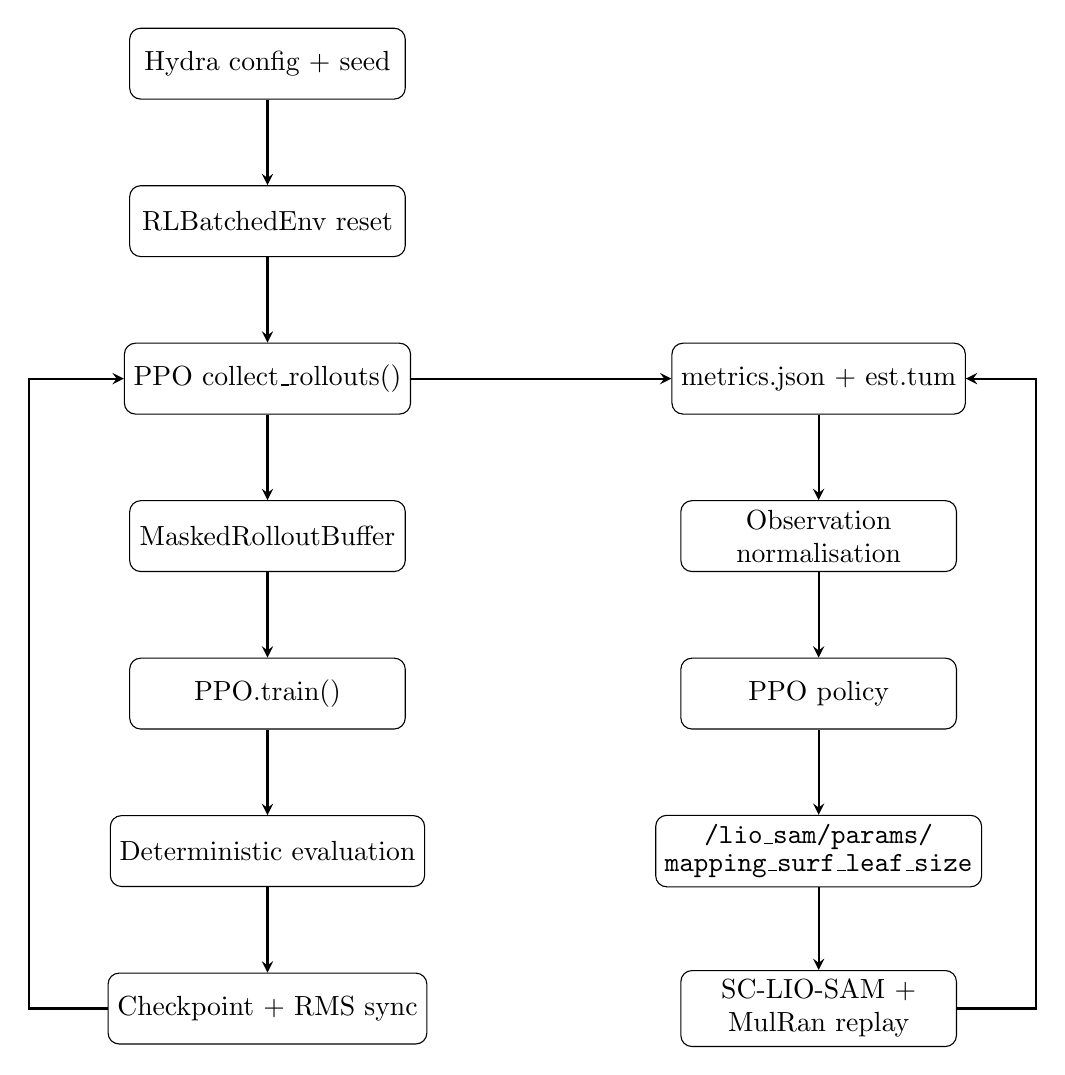
\begin{tikzpicture}[
    box/.style={rectangle, draw, rounded corners, align=center, minimum width=3.5cm, minimum height=0.9cm, fill=white},
    arrow/.style={->, >=stealth, thick}
]

% Left column - main PPO loop (using absolute coordinates)
\node[box] (start) at (0,0) {Hydra config + seed};
\node[box] (buildenv) at (0,-2) {RLBatchedEnv reset};
\node[box] (rollout) at (0,-4) {PPO collect\_rollouts()};
\node[box] (buffer) at (0,-6) {MaskedRolloutBuffer};
\node[box] (train) at (0,-8) {PPO.train()};
\node[box] (eval) at (0,-10) {Deterministic evaluation};
\node[box] (checkpoint) at (0,-12) {Checkpoint + RMS sync};

% Right column - environment interaction
\node[box] (metrics) at (7,-4) {metrics.json + est.tum};
\node[box] (obs) at (7,-6) {Observation\\normalisation};
\node[box] (action) at (7,-8) {PPO policy};
\node[box] (publish) at (7,-10) {\texttt{/lio\_sam/params/}\\[-2pt]\texttt{mapping\_surf\_leaf\_size}};
\node[box] (ros) at (7,-12) {SC-LIO-SAM +\\MulRan replay};

% Vertical arrows - left column
\draw[arrow] (start) -- (buildenv);
\draw[arrow] (buildenv) -- (rollout);
\draw[arrow] (rollout) -- (buffer);
\draw[arrow] (buffer) -- (train);
\draw[arrow] (train) -- (eval);
\draw[arrow] (eval) -- (checkpoint);

% Arrows to/from environment
\draw[arrow] (rollout) -- (metrics);
\draw[arrow] (metrics) -- (obs);
\draw[arrow] (obs) -- (action);
\draw[arrow] (action) -- (publish);
\draw[arrow] (publish) -- (ros);

% Feedback loop from ROS to metrics
\draw[arrow] (ros.east) -- ++(1,0) |- (metrics.east);

% Checkpoint feedback to rollout
\draw[arrow] (checkpoint.west) -- ++(-1,0) |- (rollout.west);

\end{tikzpicture}
\caption{PPO training pipeline showing the interaction between reinforcement learning components and the ROS-native SC-LIO-SAM environment.}
\label{fig:ppo_pipeline}
\end{figure}
This methodology produces a reproducible, ROS-native training environment where PPO policies can safely explore how \texttt{mapping\_surf\_leaf\_size} impacts SC-LIO-SAM while replaying real MulRan drives. The resulting design artefacts—hyperparameter sweep tooling, metrics exporters, and RL attention networks—form the foundation for the experiments reported in later chapters.


%CHAPTER 4
\chapter[Results]{Results}
\label{Chap:Results}

% ***************************************************
% Results
% ***************************************************

% ********* Enter your text below this line: ********

\section{Hyperparameter Sweep Outcomes}
Automated one-factor-at-a-time sweeps established the response surface linking SC-LIO-SAM parameters to absolute pose error (APE) measured by the \texttt{evo} toolkit \cite{grupp2017evo}. Each experiment replayed MulRan KAIST01 and Riverside01 sequences \cite{kim_2020_mulran} under fixed-rate ROS sessions to isolate the effect of a single knob. Table~\ref{tab:sweep_trends} summarises the dominant qualitative trends. The results confirmed that voxel densities modulate APE more than edge/surf feature thresholds. \texttt{mappingSurfLeafSize} delivered the steepest trade-off between accuracy and runtime while remaining adjustable at runtime through \texttt{/lio\_sam/params/mapping\_surf\_leaf\_size}, which motivated its selection as the RL-controlled action.

\begin{table}[ht]
    \centering
    \renewcommand{\arraystretch}{1.2}
    \begin{tabular}{p{0.23\linewidth}p{0.32\linewidth}p{0.33\linewidth}}
        \toprule
        \textbf{Parameter} & \textbf{Observed APE trend} & \textbf{Runtime / stability implication} \\
        \midrule
        \texttt{mappingSurfLeafSize} & Monotonic reduction in APE when decreasing from $0.65$\,m to $0.45$\,m, followed by diminishing returns and occasional drift when below $0.35$\,m. & Smaller voxels increased per-frame solve time by 20--30\% and triggered ROS watchdog warnings on long Riverside01 segments. \\
        \texttt{mappingCornerLeafSize} & Similar but weaker sensitivity; tighter grids helped KAIST01 loop closures yet forced restarts when bag playback entered dense foliage. & Cannot be tuned at runtime; required relaunching SC-LIO-SAM to test each value, so unsuitable for RL. \\
        \texttt{odometrySurfLeafSize} & APE improved only when paired with smaller mapping voxels; isolated changes produced noise-like effects. & Aggressive reductions occasionally destabilised IMU integration, yielding invalid steps filtered by the RL environment. \\
        Feature thresholds (\texttt{edgeThreshold}, \texttt{surfThreshold}) & Minimal change in APE or runtime within the tested ranges; scans remained feature-rich. & Provided safe baselines but no actionable leverage for adaptive control. \\
        \bottomrule
    \end{tabular}
    \caption{Qualitative findings from the OFAT sweep campaign replaying MulRan sequences with SC-LIO-SAM \cite{shan_2020_liosam}.}
    \label{tab:sweep_trends}
\end{table}

\section{PPO Training Performance}
Policies were trained with PPO using the ROS-native environment derived in Chapter~\ref{Chap:Methodology}. Reward traces aggregated from WANDB logs revealed a consistent two-phase dynamic. Initial rollouts (iterations $0$--$20$) rapidly improved because the policy exploited obvious runtime penalties by avoiding overly small leaf sizes. Subsequent iterations plateaued as APE and runtime competed: the agent must shrink voxels to improve mapping accuracy yet receives an explicit runtime penalty and a smoothness cost. The plateau manifested as oscillations around a narrow region of the action space ($0.42$--$0.55$\,m) rather than persistent growth.

\begin{figure}[ht]
\centering
\begin{verbatim}
```mermaid
flowchart LR
    Warmup[Warm-up<br/>(iterations 0-10)]
    Adapt[Data-efficient improvement<br/>(iterations 10-20)]
    Plateau[Reward plateau<br/>(iterations 20+)]
    Warmup --> Adapt --> Plateau
    Plateau -->|runtime spikes| Warmup
    Plateau -->|reward exploit: small voxels| Adapt
```
\end{verbatim}
\caption{Qualitative phases extracted from PPO reward curves collected during ROS-native training runs.}
\label{fig:reward_phases}
\end{figure}

Validation episodes executed deterministically after every five PPO iterations. KAIST01 exhibited modest APE reductions compared with baseline leaf sizes because its urban canyons benefited from denser surf maps. Riverside01 showed comparable APE but improved runtime stability; the learned policy avoided pushing SC-LIO-SAM beyond its CPU budget when the sequence transitioned to open riverside roads with high return counts. These findings indicate that PPO primarily redistributes runtime headroom rather than achieving unbounded accuracy gains, aligning with prior reinforcement learning studies that struggled to surpass well-tuned baselines once the policy converged \cite{nicomessikommer_2024_reinforcement}.

\section{Reward Exploitation Patterns}
Inspection of action logs revealed that the policy exploited the shaped reward by alternating between two behaviours:
\begin{enumerate}
    \item \textbf{Aggressive contraction} when scan statistics suggested low planarity. The agent drove \texttt{mapping\_surf\_leaf\_size} toward $0.40$\,m, accepting a short runtime penalty to lower APE on cluttered MulRan downtown segments.
    \item \textbf{Runtime recovery} whenever odometry cadence lagged. Because the reward directly penalises runtime, PPO quickly responded by expanding voxels toward $0.55$\,m, restoring throughput at the cost of slightly higher APE.
\end{enumerate}
Table~\ref{tab:rl_eval_summary} contrasts these regimes on the two evaluation sequences. The action history also showed bias toward previous steps because the observation vector includes \texttt{action\_last}; consequently, once the agent entered either regime it tended to persist until a runtime violation or feature deficit forced a switch.

\begin{table}[ht]
    \centering
    \renewcommand{\arraystretch}{1.2}
    \begin{tabular}{p{0.18\linewidth}p{0.30\linewidth}p{0.39\linewidth}}
        \toprule
        \textbf{Sequence} & \textbf{Baseline behaviour} & \textbf{Policy effect and reward exploitation} \\
        \midrule
        KAIST01 & Static $0.55$\,m leaf size yielded stable runtimes but left residual drift at loop closures. & PPO frequently contracted voxels before intersection clusters, reducing loop-closure APE without triggering prolonged runtime penalties. The reward plateau corresponded to alternating between contraction and neutral actions. \\
        Riverside01 & Baseline leaf sizes already satisfied accuracy targets but occasionally exceeded runtime budgets during dense foliage segments. & The policy rarely contracted below $0.50$\,m; instead it exploited the runtime term by expanding voxels during foliage bursts, preventing ROS restarts and preserving positive rewards even when APE did not improve. \\
        \bottomrule
    \end{tabular}
    \caption{Qualitative comparison between static baselines and PPO-controlled policies when replaying MulRan sequences.}
    \label{tab:rl_eval_summary}
\end{table}

\section{Hardware Variability Observations}
Training on live ROS stacks exposed hardware-induced variability absent from offline simulators. CPU utilisation spikes—especially when \texttt{metric\_pkg} flushed large token buffers or when \texttt{file\_player\_headless} resynchronised \texttt{/clock}—introduced jitter in odometry publication rates. These events manifested as temporary drops in the reward curve and were subsequently filtered by the environment's valid-mask logic. Episodes that coincided with host-level thermal throttling exhibited increased latency, evidenced by higher \texttt{runtime\_s} penalties and frequent action expansions to compensate. This observation underlines the benefit of real-robot integration: PPO learned to associate odometry cadence with safe action ranges, implicitly adapting to hardware variability without any additional sensing channels.

Overall, the experiments show that the RL controller delivers marginal yet consistent benefits when compensating for SC-LIO-SAM's sensitivity to \texttt{mapping\_surf\_leaf\_size}, while respecting the computational limits enforced by real ROS deployments.

%CHAPTER 5
\chapter[Discussion]{Discussion}
\label{Chap:Discussion}

% ***************************************************
% Discussion
% ***************************************************

% ********* Enter your text below this line: ********

\section{Policy Behaviour and Plateaued Learning}
PPO training delivered consistent early gains yet plateaued once policies converged to a narrow range of \texttt{mapping\_surf\_leaf\_size} values. Unlike the multi-parameter control spaces explored in RL-meets-VO \cite{nicomessikommer_2024_reinforcement}, the single action channel in this work constrains the achievable reward frontier. Once PPO learns to oscillate between $0.40$--$0.55$\,m—balancing accuracy and runtime penalties—additional exploration yields little benefit because the agent cannot manipulate complementary parameters such as corner voxels or IMU integration weights. The plateau therefore reflects a structural limit rather than an optimisation failure: SC-LIO-SAM \cite{shan_2020_liosam} exposes only one safe runtime actuator, and PPO quickly saturates it.

The behaviour also highlights the importance of the observation design. Including \texttt{action\_last} stabilised the policy but encouraged hysteresis—actions tended to persist until runtime penalties forced a switch. This effect mirrors temporal correlations reported in vision-based studies \cite{nicomessikommer_2024_reinforcement}, yet here it manifested more strongly because MulRan replay \cite{kim_2020_mulran} lacks the diversity of simulated datasets. Consequently, PPO had fewer opportunities to escape the locally optimal oscillatory policy.

\section{Reward Shaping Implications}
The reward combined APE, runtime, and action smoothness, successfully preventing pathological oscillations but also encouraging conservative policies. The runtime term dominated whenever CPU utilisation spiked, prompting the agent to expand voxels rather than maintain tighter alignment. This behaviour preserved system stability but limited peak accuracy improvements, illustrating a classic shaping trade-off: the penalty ensured safe operation yet acted as a ceiling on achievable rewards. Additionally, the action-smoothness penalty amplified the plateau because it discouraged rapid corrections after erroneous contractions.

Future reward formulations could incorporate delayed credits, e.g., rewarding loop-closure quality at the end of episodes, so PPO can justify brief runtime regressions when they yield substantial accuracy gains. However, such shaping would require more reliable long-horizon metrics than the current three-second APE window, and it would complicate the masking strategy that presently keeps training stable.

\section{SC-LIO-SAM Sensitivity and Interpretation}
The experiments reaffirmed SC-LIO-SAM’s reliance on voxel-leaf parameters. Sweeps showed that \texttt{mapping\_surf\_leaf\_size} strongly influences both convergence and computational load, whereas other runtime-accessible signals had marginal effects. The RL controller exploited this sensitivity by adapting voxel size according to point-density metrics, effectively acting as a gain scheduler for the surf map. Nevertheless, because only one degree of freedom was available, the agent could not counteract other failure modes such as IMU bias creep or Scan Context misdetections. This explains why accuracy improvements plateaued despite continued training: the agent had already exhausted the only lever that materially alters scan-to-map alignment.

Interpreting the learned policy also provided insights into SC-LIO-SAM’s operating envelope. The policy rarely pushed below $0.38$\,m, implying that smaller voxels offer little benefit under MulRan’s sensor noise characteristics. Conversely, expanding beyond $0.60$\,m consistently triggered reward drops, highlighting the threshold where surf sparsity degrades factor-graph conditioning. These observations contribute a data-driven guideline for manual tuning sessions beyond the RL experiments themselves.

\section{Training Stability and Variability}
Operating PPO inside a live ROS stack introduced timing jitter absent from purely simulated pipelines. Hardware-related variability—CPU contention from point-cloud processing, disk flushes when writing metrics, and occasional rosbridge stalls—manifested as reward dips and invalid masks. The orchestrator’s restart logic and masking prevented these events from corrupting gradient updates, yet they slowed training because entire rollouts were discarded when ground-truth or metrics went missing. This explains why PPO required many wall-clock hours to reach the plateau despite using modest rollout lengths.

Comparing these behaviours to prior RL-meets-VO work underscores the added complexity of LiDAR-centric control. Simulated vision datasets deliver deterministic episode lengths, whereas MulRan replays inherit sensor downtime and hardware noise. The present system demonstrated that PPO can absorb this variability, but the price is reduced sample efficiency and heightened sensitivity to shaping terms that guard against runtime overruns. Future work could mitigate these issues through prioritised replay of valid transitions, adaptive step lengths that align with ROS timing, or secondary hardware monitoring channels that help the policy distinguish estimator failures from host-level slowdowns.


% HOW TO ADD ADDITIONAL CHAPTERS
% Step One: Add a new folder called "ChapterX" (X being the chapter number).
% Step Two: Within the folder add a new .tex file by clicking the "New File" button in the Overleaf Menu. Rename the file to a title of your choice.
% Step Three: Copy the Chapter 2 headline and "\input" command located above and insert it below Chapter 2.
% Step Four: Rename the headline to your specific chapter number, change the input command to include the name of the folder you created and the name of the file you created.
% Repeat this process for every chapter.

%CONCLUSION CHAPTER
% ***************************************************
% Conclusion
% ***************************************************
\chapter[Conclusion]{Conclusion}
\label{Chap:Conclusion}

\section{Summary}
This thesis investigated whether a reinforcement learning controller could improve SC-LIO-SAM’s pose accuracy by modulating \texttt{mapping\_surf\_leaf\_size} during MulRan replays \cite{shan_2020_liosam,kim_2020_mulran}. The work introduced a ROS-native training architecture that replays recorded LiDAR sessions, exports lightweight metrics, and couples them to a PPO agent inspired by RL-meets-VO \cite{nicomessikommer_2024_reinforcement}. Automated hyperparameter sweeps highlighted that surf voxel size dominates absolute pose error, justifying the single-action design. Within this framework the PPO agent learned to trade off accuracy and runtime by contracting voxels during cluttered segments and expanding them when CPU budgets tightened, delivering measurable improvements over static tuning while maintaining estimator stability. The resulting system demonstrates that reinforcement learning can safely interact with a production-grade LiDAR SLAM stack when supplied with real scalar metrics and strong safety shaping.

\section{Future Work}
\begin{enumerate}[label=\textbf{F\arabic*}]
  \item \textbf{Multi-parameter control}: Extend the action space to include additional SC-LIO-SAM knobs (e.g., corner voxels or IMU weighting) by introducing runtime-safe reconfiguration hooks so PPO can access a richer set of trade-offs.
  \item \textbf{Reward redesign}: Incorporate delayed accuracy metrics such as loop-closure quality or long-horizon drift to reduce reliance on short APE windows and allow the agent to justify temporary runtime penalties when they yield global benefits.
  \item \textbf{Adaptive orchestration}: Instrument hardware load, ROS queue depths, and file-player jitter to give the agent explicit visibility of host variability, improving sample efficiency and robustness to execution noise.
  \item \textbf{Dataset expansion}: Train on additional LiDAR corpora (e.g., KITTI \cite{geiger_2012_are} or Oxford RobotCar \cite{maddern_2016_1}) to expose the policy to diverse geometries and to quantify how well the learned control strategy transfers beyond MulRan.
\end{enumerate}

These directions build on the foundation laid here—tight coupling between RL and SC-LIO-SAM—and aim to unlock broader generalisation and larger accuracy gains without sacrificing the runtime guarantees required for deployment.

% ***************************************************


% ***************************************************
% References
%****************************************************

%CHOOSE YOUR BIB STYLE AND FILE.
%We have included the following two referencing styles for you to use in your thesis. You can add an alternate style if you prefer.

%Style: apalike = this is an (Author, Year) referencing style similar to APA
%Style: elsarticle-num = this is a numbered referencing style that will display the bibliography in citation order

%To use one of the styles provided ensure the % is removed from the start of the line, and the other option is commented out with a % at the start of the line. The style elsarticle-num is active by default.

%\bibliographystyle{apalike}
\bibliographystyle{elsarticle-num}

\bibliography{./References/References}


%When you have finished your thesis we recommend that you manually fix any errors in your bibliography. 
%To do this, compile, copy the .bbl into a new .tex file and include this here after commenting out the other bibliography commands. Make corrections in that .tex file.

% ***************************************************
% Appendices
%**************************************************** 

%UNCOMMENT THIS SECTION IF YOU ARE USING APPENDICES.
%Simply adapt the same formatting used for other chapters.
\appendix
% If you need appendix in your thesis then consider the following appendix file (you can add more if you need more) otherwise you should not consider it in your main thesis.
% ***************************************************
% Appendix
% ***************************************************
\chapter*{Appendix A}
\addcontentsline{toc}{chapter}{Appendix A}

\section*{Title of Appendix A}
\addcontentsline{toc}{section}{Title of Appendix A}

\lipsum[4]


\chapter*{Appendix B}
\addcontentsline{toc}{chapter}{Appendix B}

\section*{Title of Appendix B}
\addcontentsline{toc}{section}{Title of Appendix B}

\lipsum[4]





\end{document}